\section{Basic concepts}
\subsection{Basic data structure}
StreamNet is a Directed Acyclic Graph, where each vertex in the $DAG$ represents a block and the directed edge represents a confirmation relationship between blocks.
For instance, vertex $0$ in Figure~\ref{simple_sn} represents the Genesis block, which is by default a confirmed block.
Vertex $1$, on the other hand, represents the first block, which is confirmed by the subsequent block $2$, $3$ and $4$. 
When a new block is not confirmed, it is called a tip. For example, in Figure~\ref{simple_sn}, block $6$ is a tip.

\begin{figure}[!ht]
\begin{center}
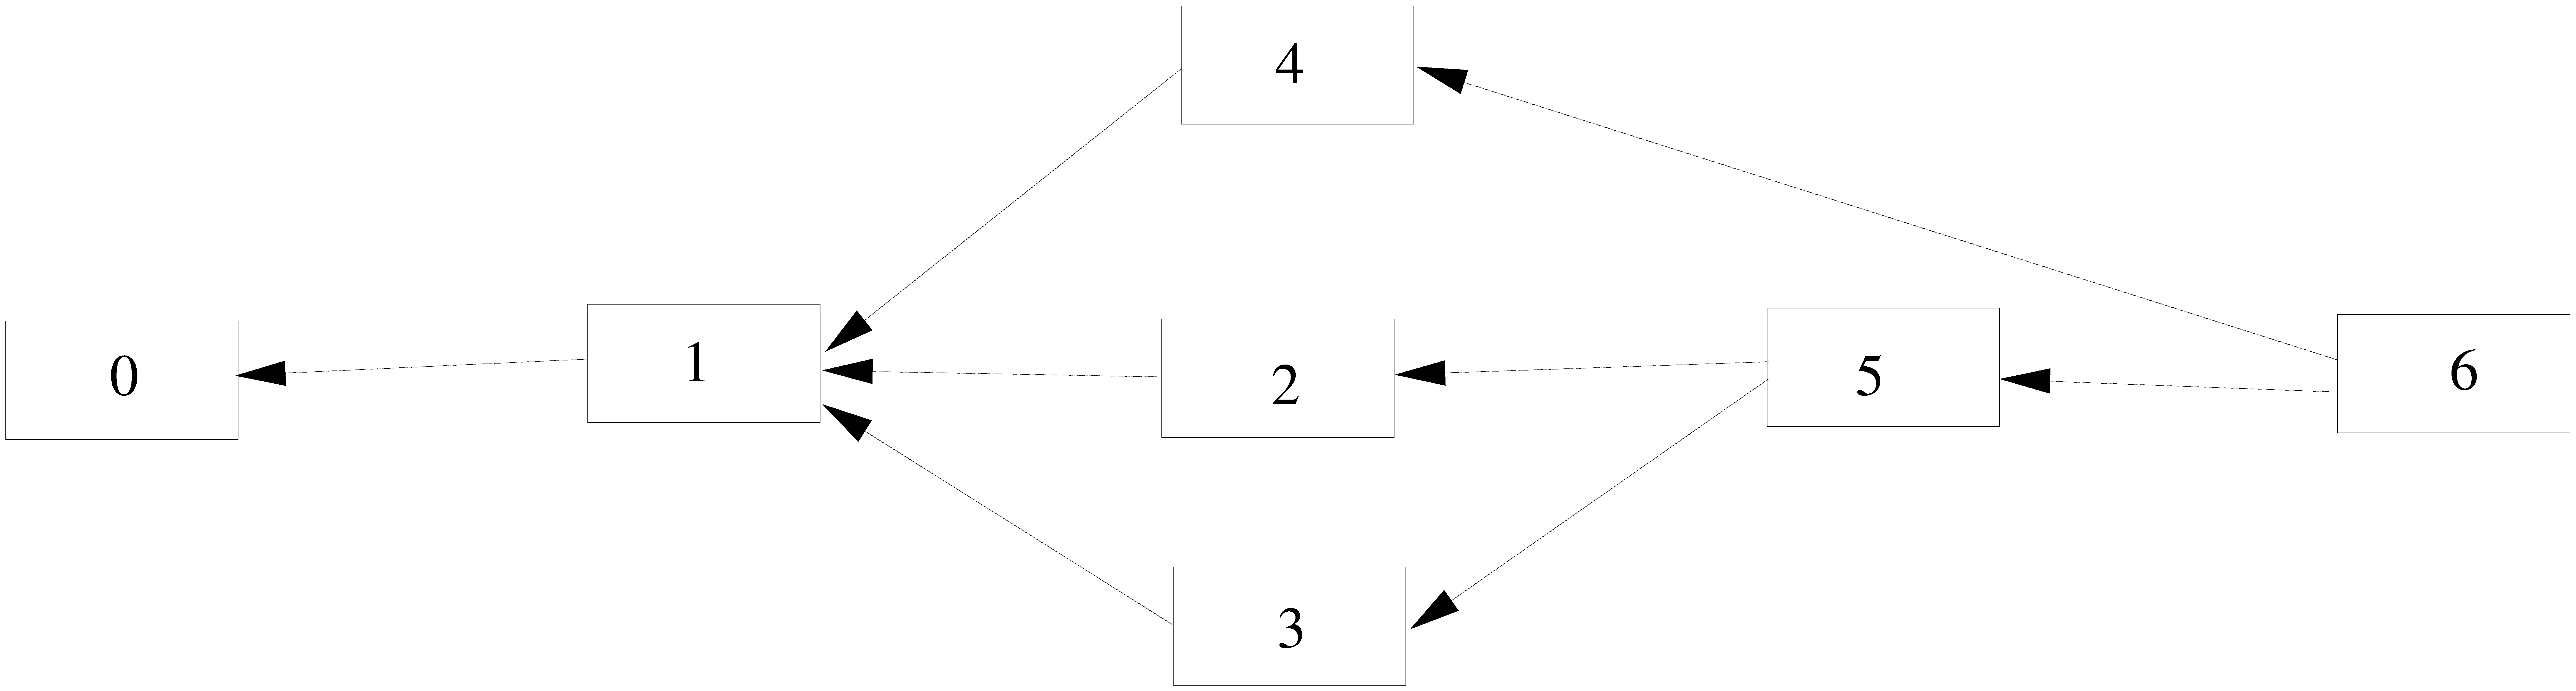
\includegraphics[width=0.45\textwidth]{figures/simple_sn.eps}
    \caption{
        Example of the StreamNet data structure.
     }
\label{simple_sn}
\end{center}
\end{figure}



\subsection{Transaction}
\subsubsection{Genesis transaction}

\begin{figure}[!ht]
\begin{center}
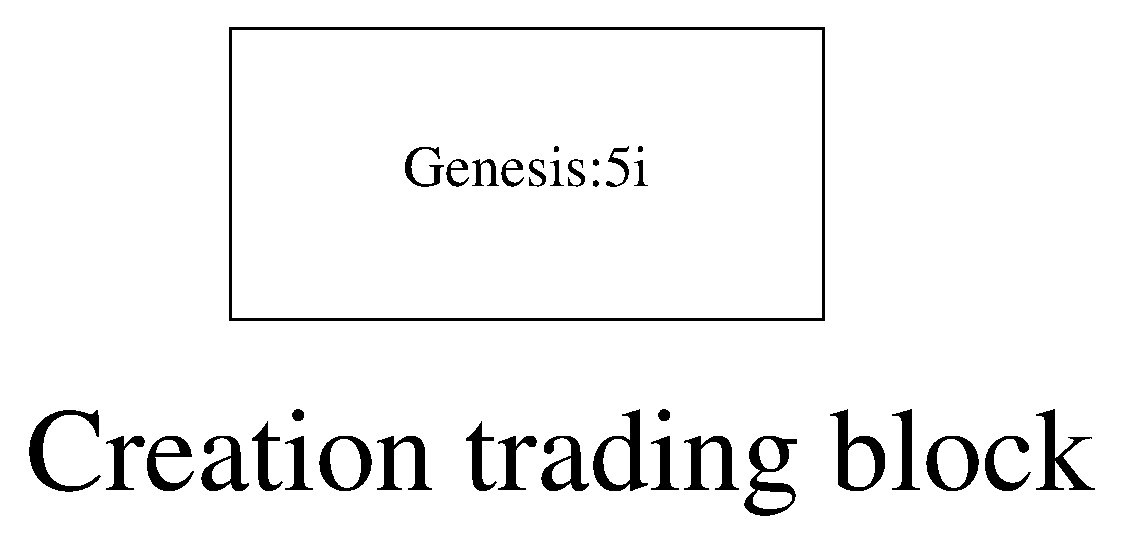
\includegraphics[width=0.15\textwidth]{figures/genesis.eps}
    \caption{
        The creation of genesis node.
     }
\label{genesis}
\end{center}
\end{figure}

There is no concept of mining in StreamNet, and all tokens are included in the Genesis Node.
In Figure~\ref{genesis}, an initial transaction is created with $5$ tokens.


\subsubsection{Transaction Content}

\begin{figure}[!ht]
\begin{center}
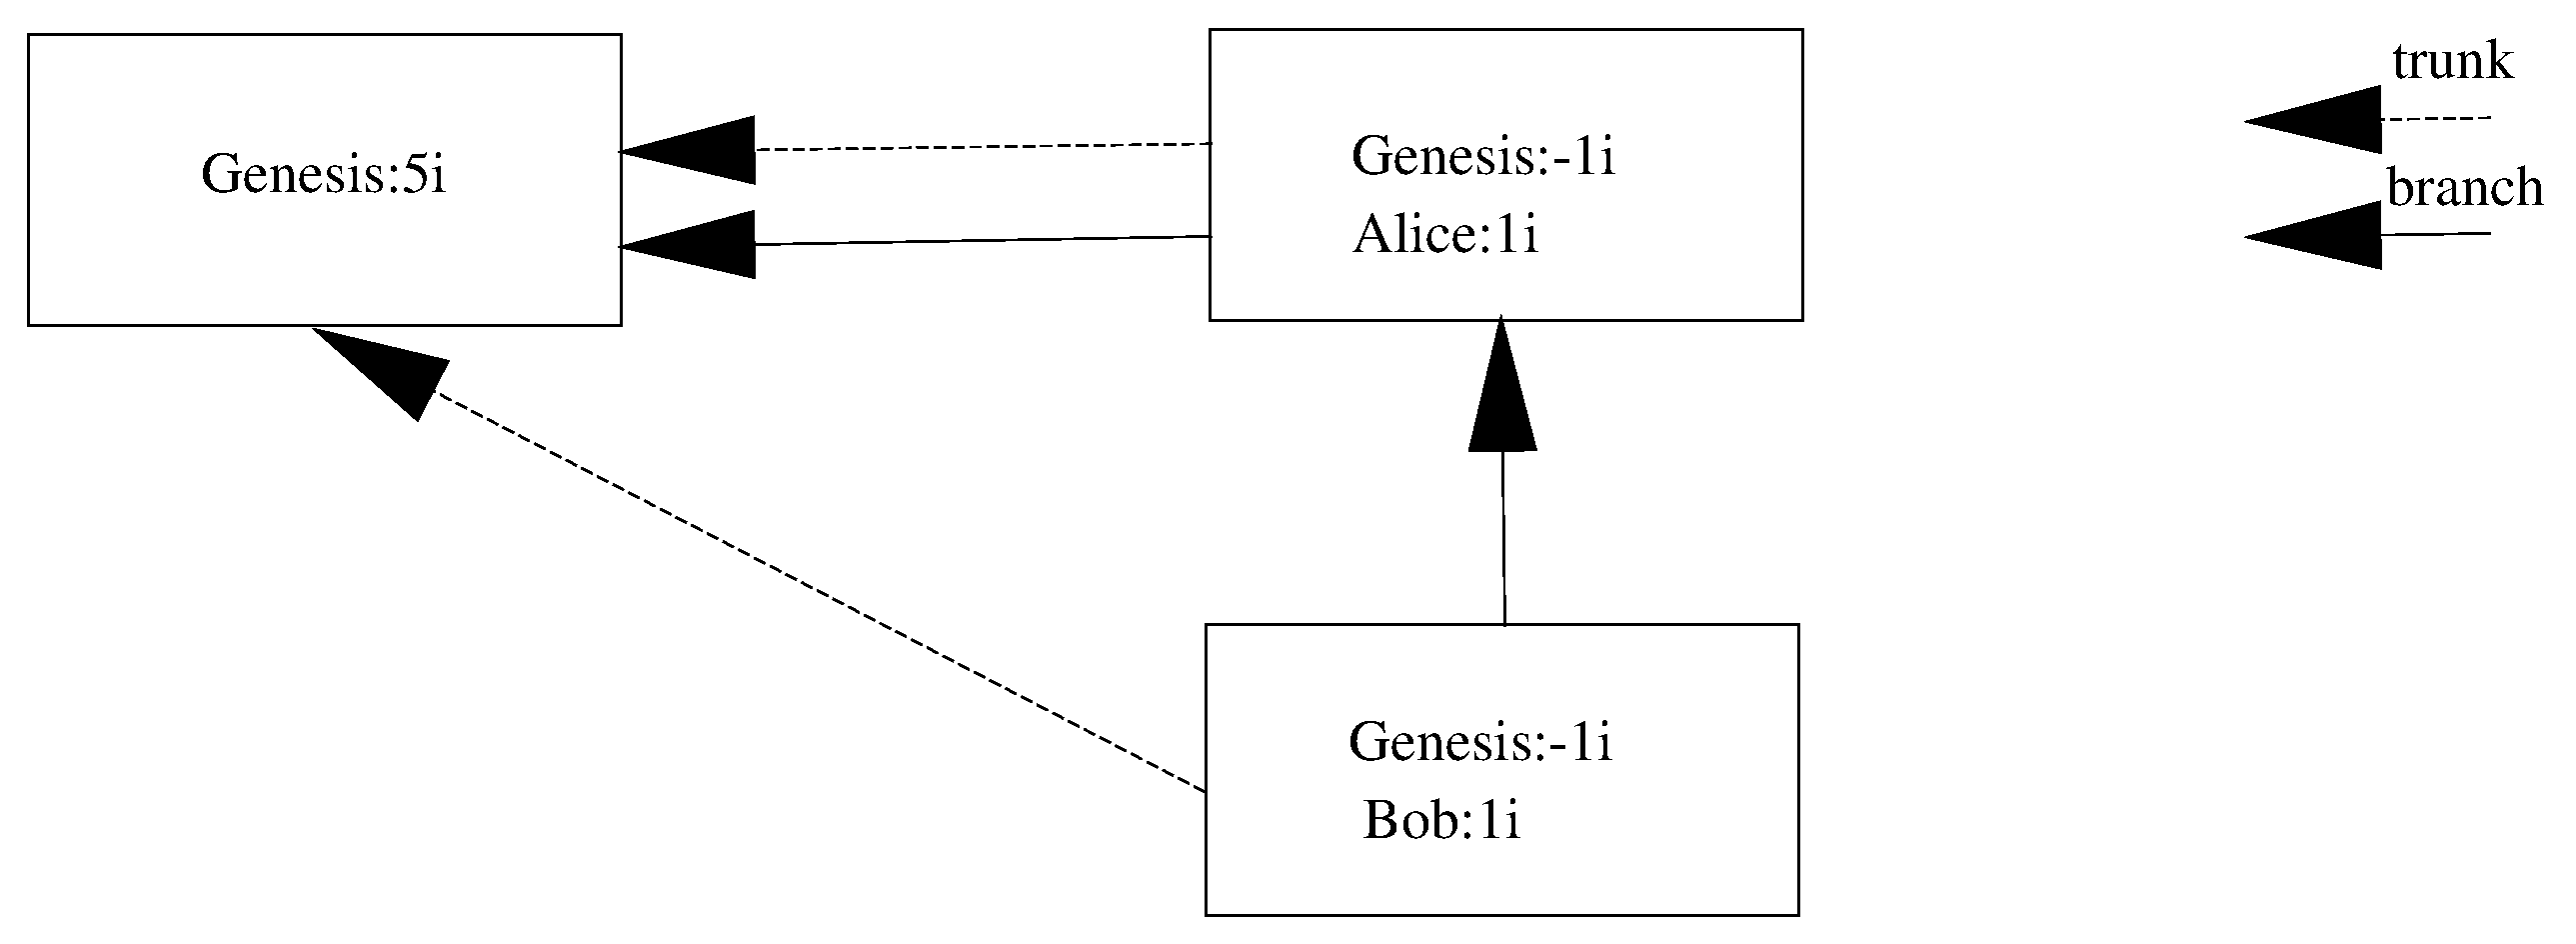
\includegraphics[width=0.35\textwidth]{figures/simple_transfer.eps}
    \caption{
        An example of token transfers.
     }
\label{simple_transfer}
\end{center}
\end{figure}

Assume that in Figure~\ref{genesis}, Genesis wants to transfer $1$ token to Alice, 
and then hopes to transfer $1$ token to Bob and attach the transaction node to StreamNet, the resulting $DAG$ is shown in Figure~\ref{simple_transfer}.
Here, each transaction must find two tip transactions to confirm, namely trunk and branch transactions.
For example, the Genesis $\rightarrow$ Alice transaction confirms the Genesis transaction itself,
while the Genesis $\rightarrow$ Bob transaction confirms the Genesis transaction and the Genesis $\rightarrow$ Alice transaction.
When a transaction wants to be attached to StreamNet, it must do enough Proof of Work (POW),
but this POW differs from Bitcoin in that its difficulty is fixed and therefore does not need the participation of miners.

\subsubsection{Transaction validation (approve)}

\begin{figure}[!ht]
\begin{center}
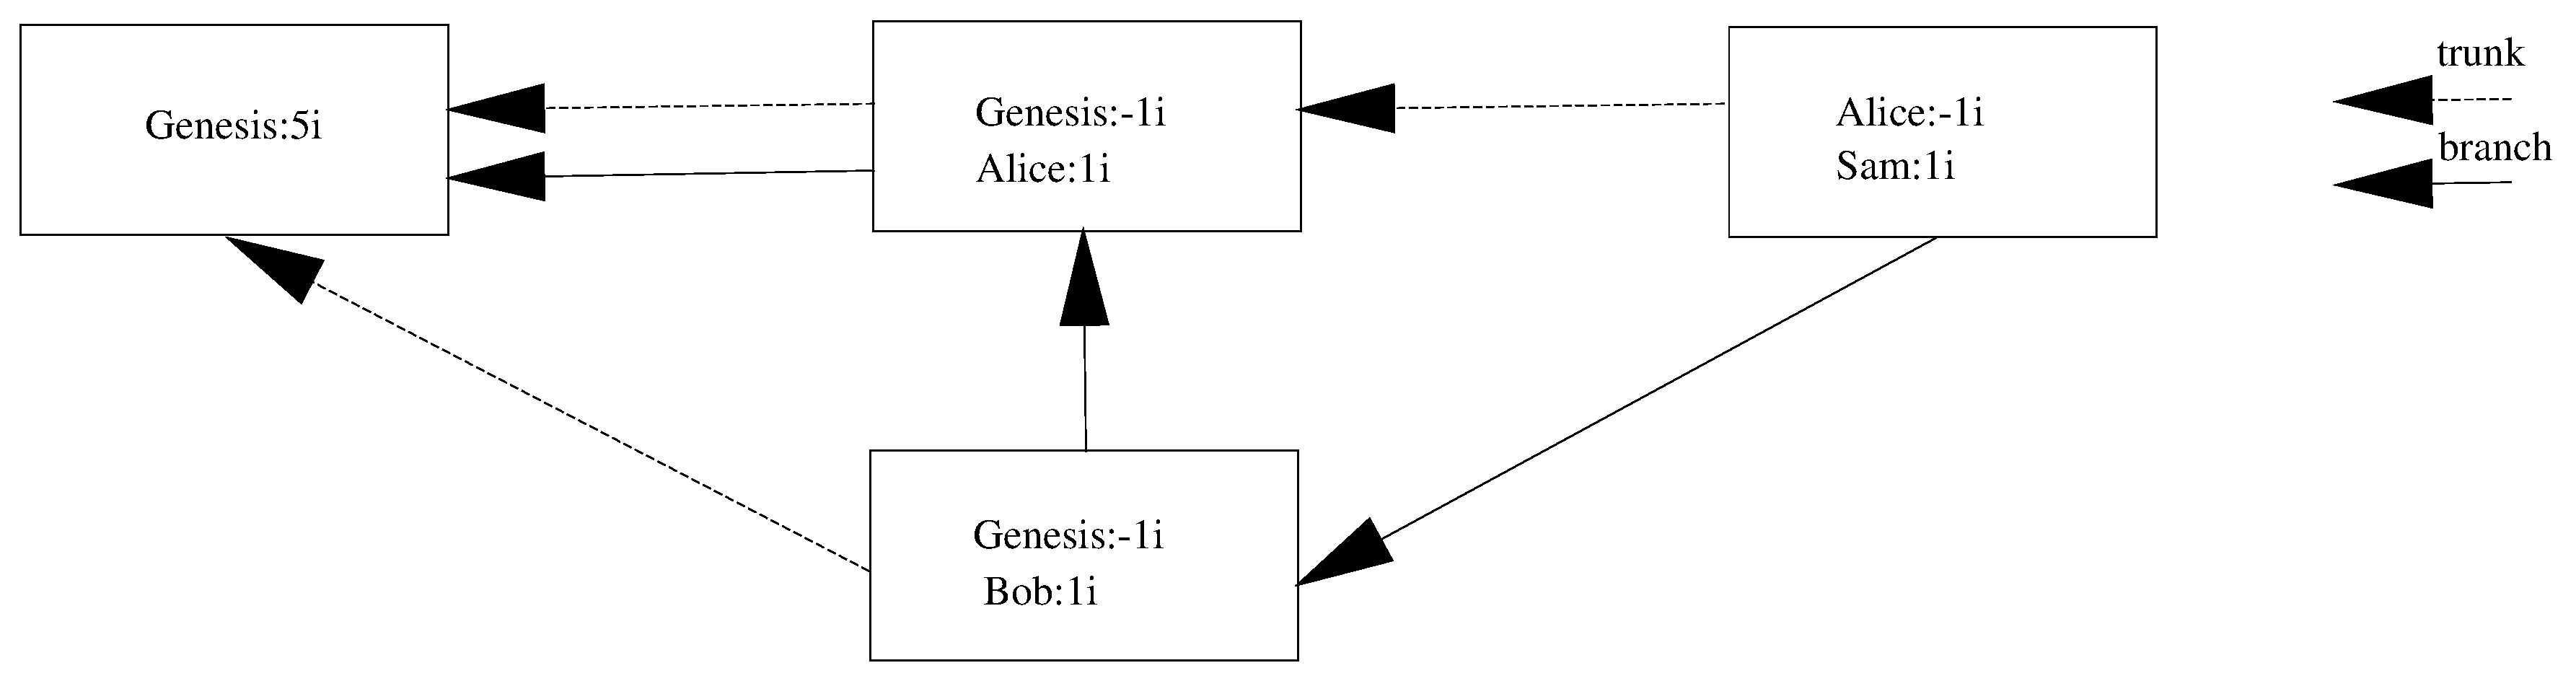
\includegraphics[width=0.35\textwidth]{figures/txn_success.eps}
    \caption{
        An example of succesfull token transfer.
     }
\label{txn_success}
\end{center}
\end{figure}

Because a new transaction needs to find two tip transactions to approve, the validation process is diveded into two steps:

\begin{itemize}
\item Start from Genesis, verify all transactions that are directly or indirectly referenced, 
mainly to see if this will result in a negative balance or loss of the token \cite{gal_2018}.
For example, in Figure~\ref{txn_success}, the Alice $\rightarrow$ Sam transfer needs to validate transactions it indirectly or directly approves.
It constructs a topological transfer sequence, 
namely (Genesis) $\rightarrow$ (Genesis $\rightarrow$ Alice) $\rightarrow$ (Genesis $\rightarrow$ Bob) $\rightarrow$ (Alice $\rightarrow$ Sam),
and find that each step does not violate the principle of transfer, which means the verification is successful.
In Figure~\ref{txn_fail}, the same topology sequence, when verifying (Genesis $\rightarrow$ Bob), 
because the Genesis balance will be reduced to -1, the verification fails.
As an honest node, Alice $\rightarrow$ Sam transaction Will find a new tip to verify,
but it can also choose to cheat, attach this transaction to the selected tip.
However, it is likely to result in subsequent rejection of this transaction.
\item At the mean time, the signature of the transaction needs to be checked to ensure that the link relationship has not been tampered with.
\end{itemize}

\begin{figure}[!ht]
\begin{center}
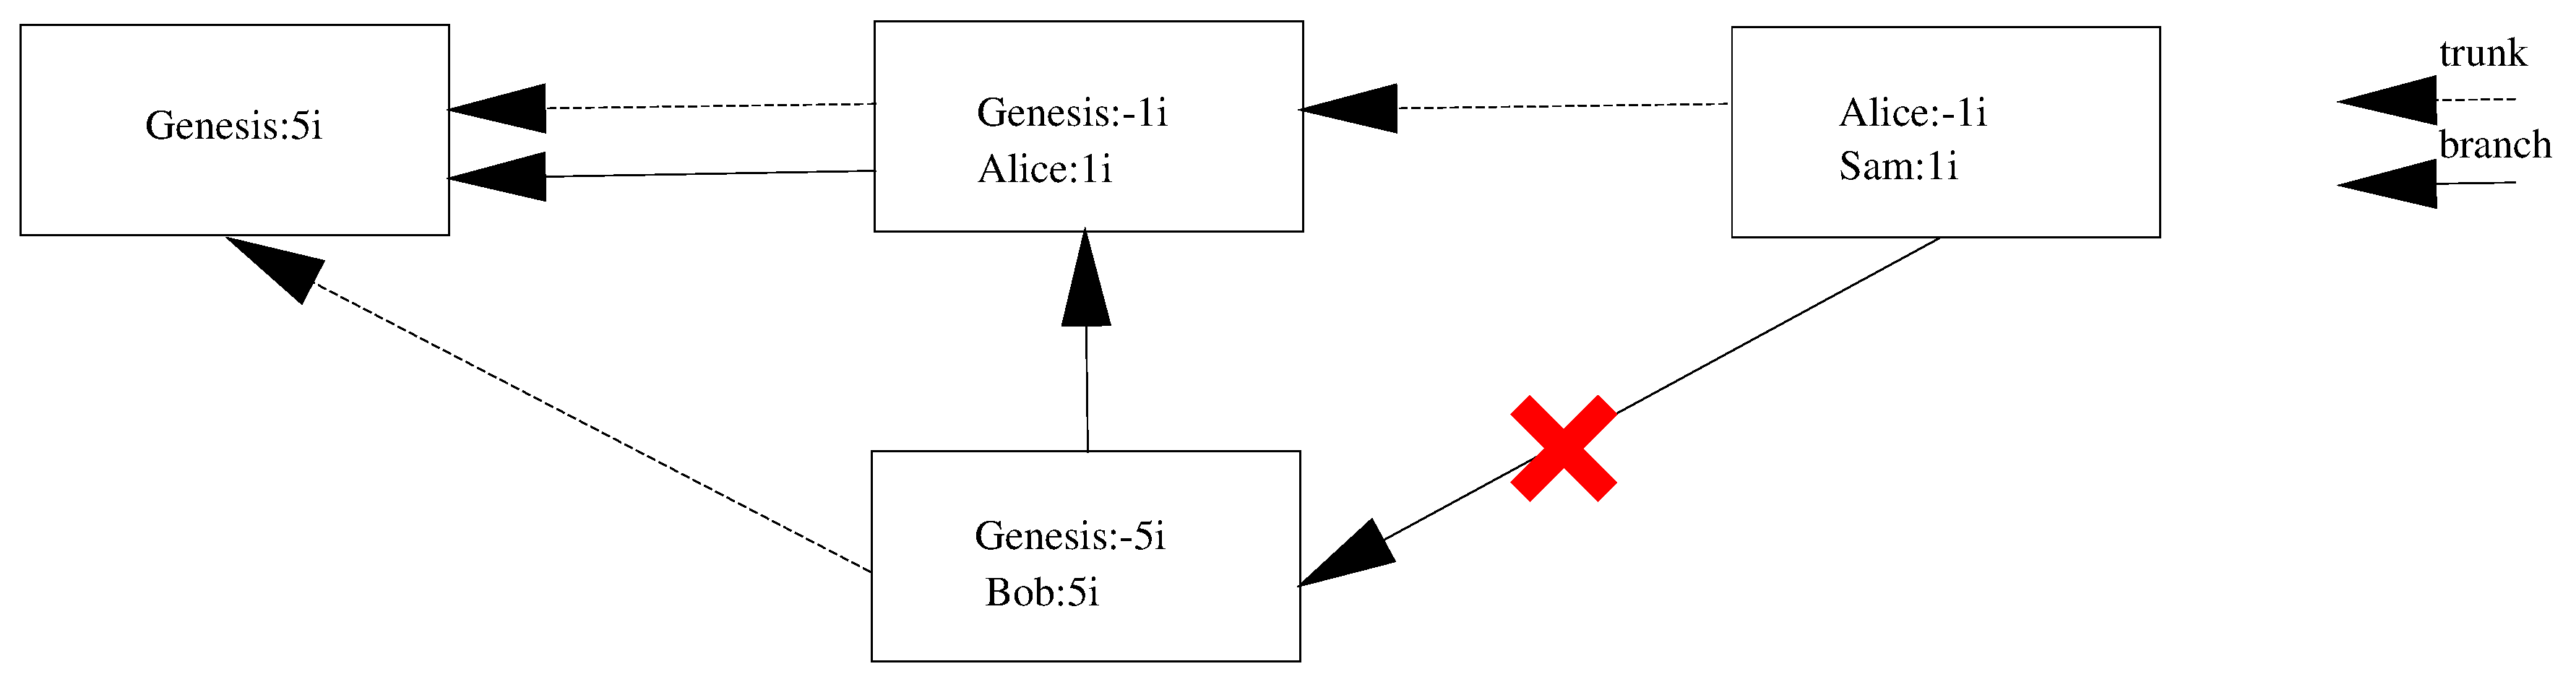
\includegraphics[width=0.35\textwidth]{figures/txn_fail.eps}
    \caption{
        An example of errornous token transfer.
     }
\label{txn_fail}
\end{center}
\end{figure}

\subsubsection{Tip Selection}
There are two basic concepts in StreamNet, one is the transaction rate $\lambda$, which indicates the number of transactions per time unit.
For convenience, we set the time unit to seconds.
The other is invisible period $h$, indicating how many time units a transaction has not been seen by other incoming blocks after attachment.
Because of $h$, the transaction rate $\lambda$ has an important influence on the shape of StreamNet.
For example, in Figure~\ref{slow_txn}, when the transaction rate is slow, StreamNet is more like a chain.
In the case of high throughput transaction in Figure~\ref{fast_txn}, the shape of StreamNet is a star.

\begin{figure}[!ht]
\begin{center}
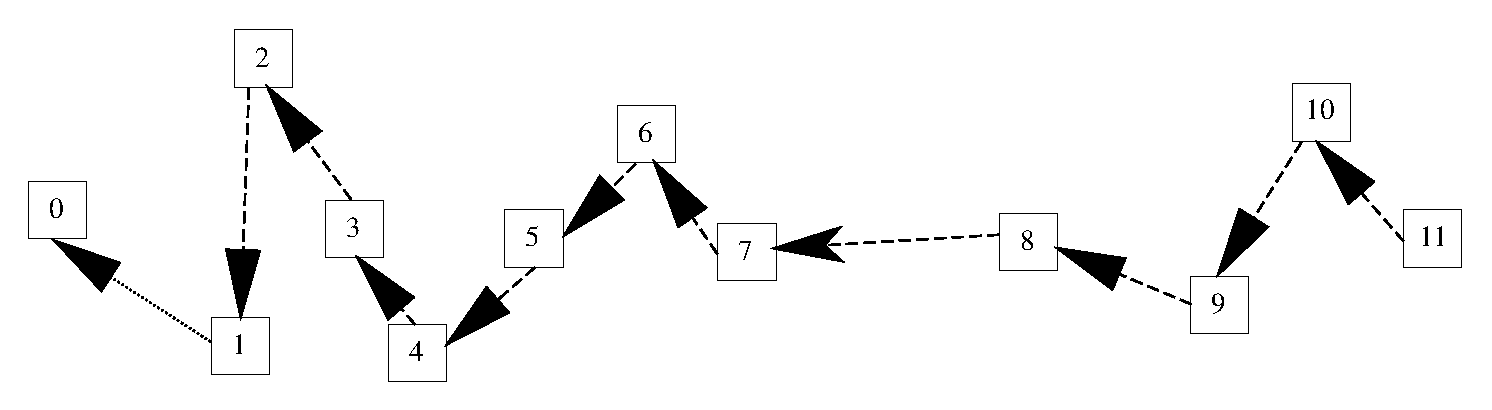
\includegraphics[width=0.35\textwidth]{figures/slow_txn.eps}
    \caption{
        The shape of StreamNet when the txn rate is low. 
     }
\label{slow_txn}
\end{center}
\end{figure}

\begin{figure}[!ht]
\begin{center}
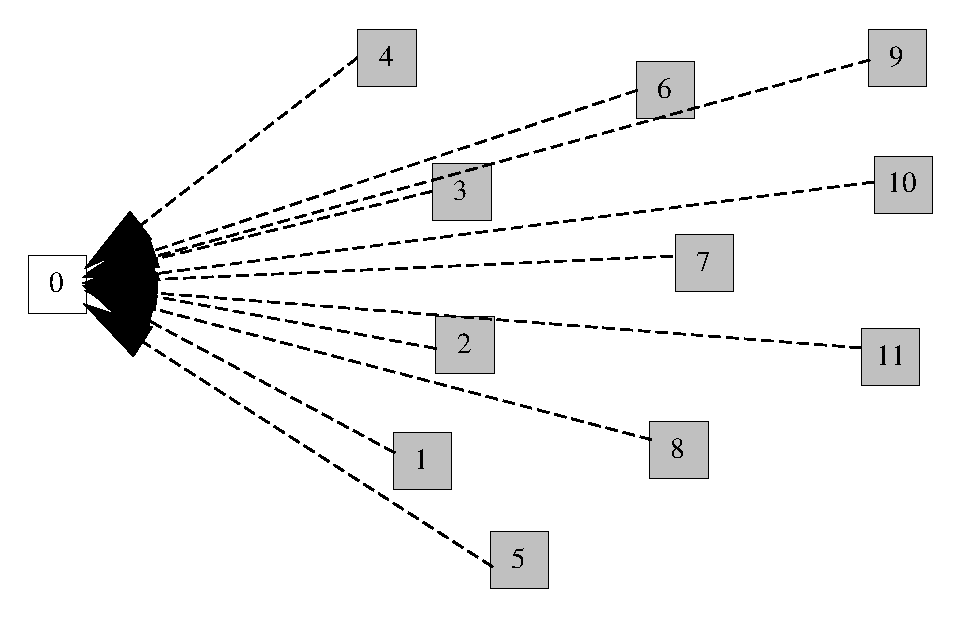
\includegraphics[width=0.35\textwidth]{figures/fast_txn.eps}
    \caption{
        The shape of StreamNet when the txn rate is high. 
     }
\label{fast_txn}
\end{center}
\end{figure}

One of simplest tip selection algorithms is the random walk with equal probability starting from Genesis, as shown in Figure~\ref{random_equal}.
Suppose Alice $\rightarrow$ Sam transaction wants to select tip, which starts from Genesis transaction.
There are two options, one is Genesis $\rightarrow$ Alice, the other is Genesis $\rightarrow$ Bob,
the probability of selecting Genesis $\rightarrow$ Alice is $\frac{1}{2}$, while Genesis $\rightarrow$ Bob is $\frac{1}{2}$. 

\begin{figure}[!ht]
\begin{center}
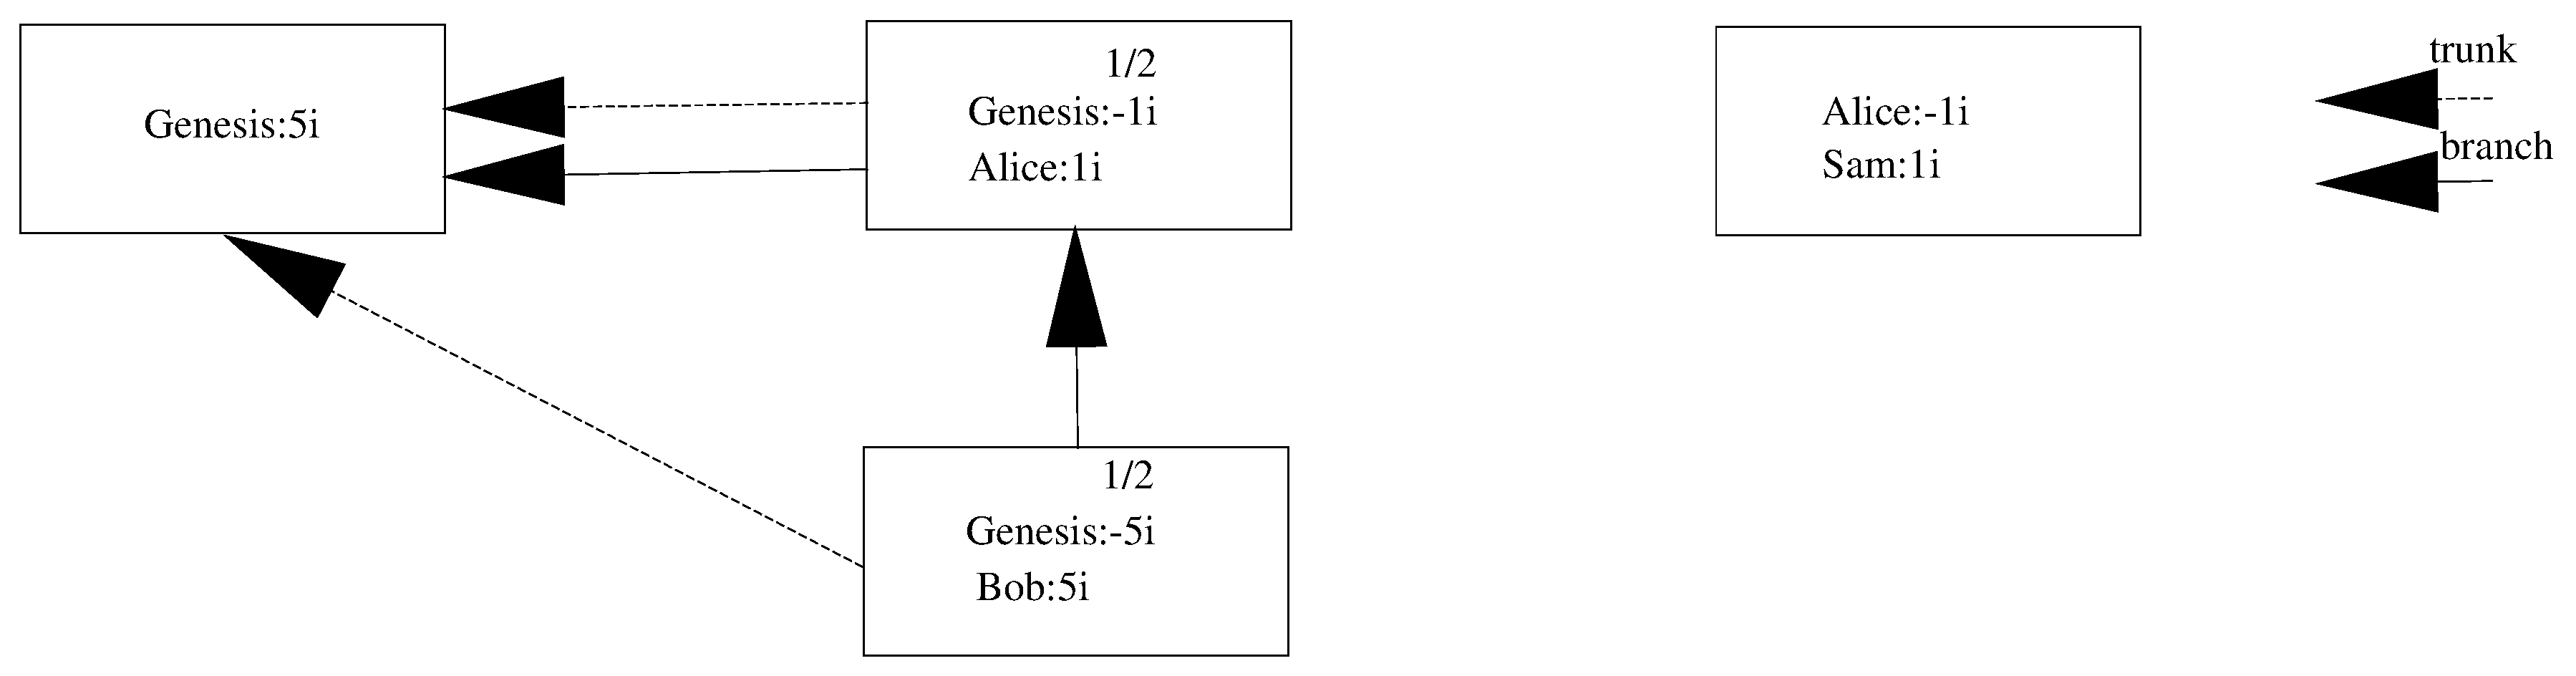
\includegraphics[width=0.35\textwidth]{figures/random_equal.eps}
    \caption{
        Random walk with equal probability.
     }
\label{random_equal}
\end{center}
\end{figure}

\begin{figure}[!ht]
\begin{center}
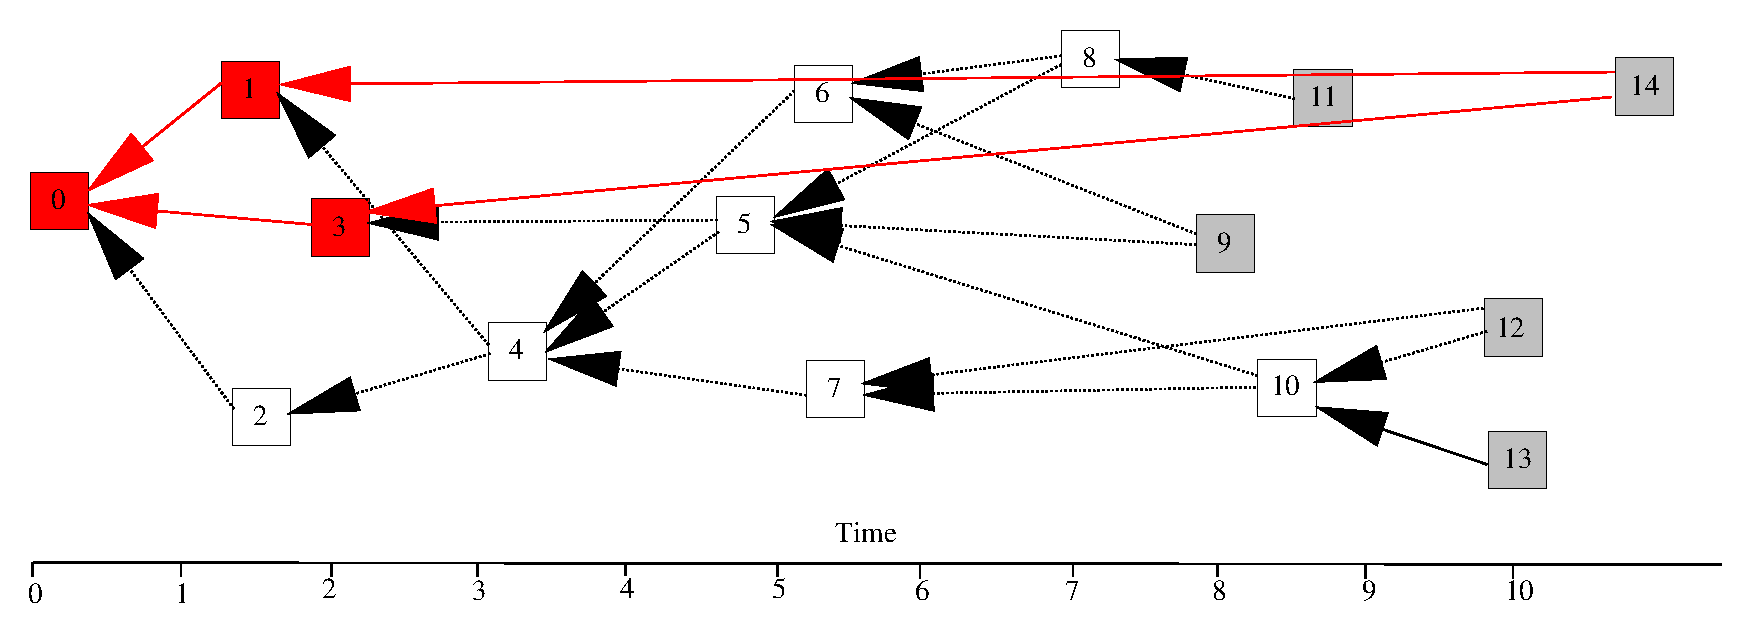
\includegraphics[width=0.35\textwidth]{figures/lazy_txn.eps}
    \caption{
        An example of lazy transaction.
     }
\label{lazy_txn}
\end{center}
\end{figure}

\begin{figure}[!ht]
\begin{center}
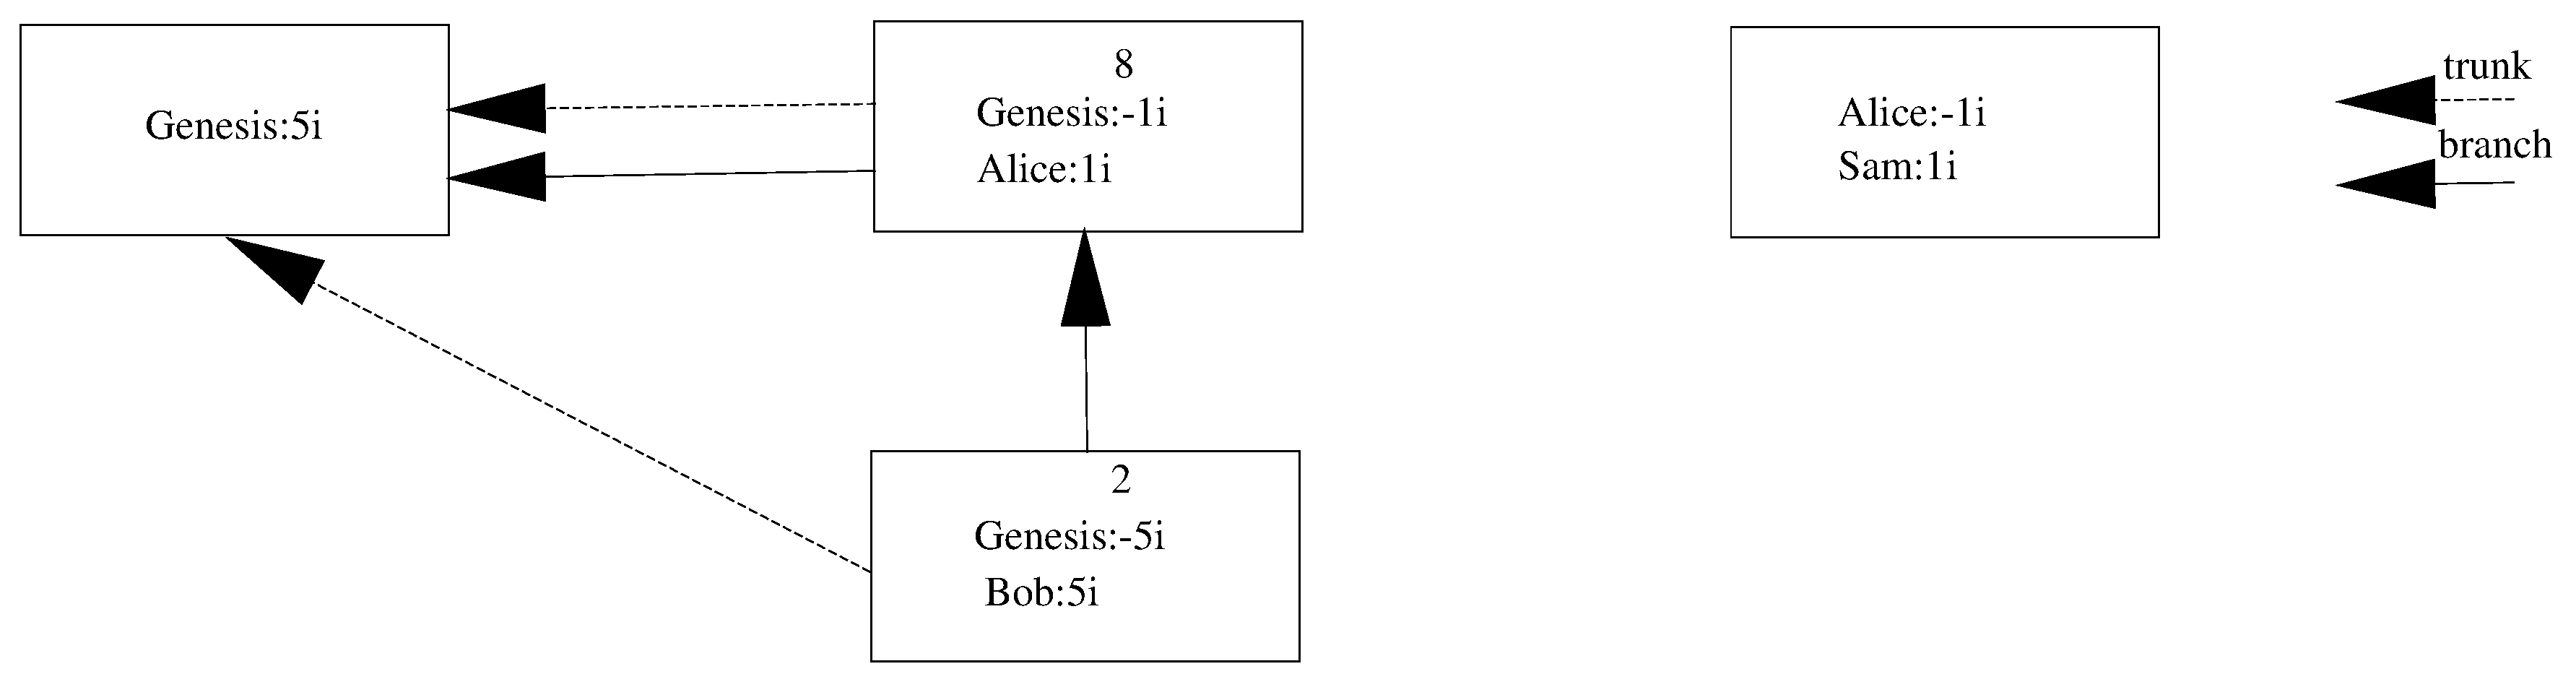
\includegraphics[width=0.35\textwidth]{figures/random_unequal.eps}
    \caption{
        Random walk with equal probability.
     }
\label{random_unequal}
\end{center}
\end{figure}

\begin{figure}[!ht]
\begin{center}
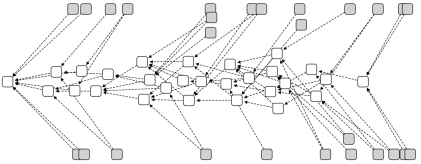
\includegraphics[width=0.35\textwidth]{figures/super_weight.png}
    \caption{
        Example of the result using super-weight algorithm.
     }
\label{super_weight}
\end{center}
\end{figure}

The problem with the simple random walk algorithm is that it produces lazy transactions.
For example, in Figure~\ref{lazy_txn}, transaction $14$ is a lazy transaction that causes new transactions to approve older transactions without being penalized.
This problem can be solved by using Monte Carlo Random Walk (MCMC).
In Figure~\ref{random_unequal}, there is a weight on both transactions, for example, Genesis $\rightarrow$ Alice is $8$, and Genesis $\rightarrow$ Bob is $2$,
then the probability of selecting Genesis $\rightarrow$ Alice is $\frac{8}{10}$,
and Genesis $\rightarrow$ Bob is $\frac{2}{10}$. 
The weight is determined by how many transactions have directly or indirectly approved the transaction.
The more approved transactions, the greater the weight.
If only weights are used then it is a super-weight algorithm, meaning that large-weight transactions are always preferred.
The problem with this algorithm is that there are many transactions that can never be confirmed.
Figure~\ref{super_weight} shows the results of a super-weighted algorithm. 
If purely using probability weighting, then it is a
super-probability algorithm. The trade-off between the two is represented by a $\alpha$, and it can be considered that the
larger the $\alpha$ is, the smaller the randomness is.
The method of specifically using $\alpha$ to calculate the jump probability is expressed in the formula (1).
Which represents the weight of the trading node.Where $P_{xy}$ represents the probability of jumping from $x$ to $y$. $H_{y}$ represents the weight of the trading node $y$.

\begin{equation}
\label{simple_equation}
P_{xy} = \frac{e^{\alpha H_{y}}}{\Sigma_{z:z \rightarrow x}e^{\alpha H_{z}}}
\end{equation}

\subsubsection{Transaction Consensus in the Gossip network}

\begin{figure*}[ht]
\begin{center}
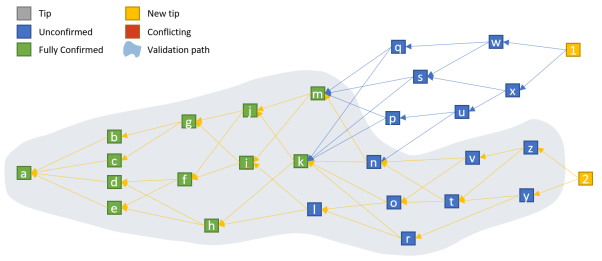
\includegraphics[width=0.65\textwidth]{figures/full_confirmation.png}
    \caption{
        Example of fully confirmed transactions.
     }
\label{full_confirmation}
\end{center}
\end{figure*}

There are currently three ways to confirm a transaction in StreamNet:
\begin{itemize}
\item The first way is that the common nodes covered by all the previous tips are considered to be fully confirmed; for example, in Figure~\ref{full_confirmation}, 
    the nodes referenced or indirectly referenced by tip1 are blue and yellow line covered transactions, 
    while the tip2 reference Or the indirectly referenced node is a yellow line covered transaction.
    If there are only 1, 2 tips in StreamNet, then the green node is a fully confirmed transaction, while the green node is an unconfirmed transaction.
\item The second way is that the system sends a Coordinator tip every 1 minute.
    This tip is called milestone and is attached to StreamNet.
    All transactions referenced by this Coordinator tip are confirmed.
\item The third way is to use Monte Carlo Random Walk (MCMC). 
    Call N times to select a tip using the tip selection algorithm.
    If a block is referenced by this tip, its credibility is increased by 1.
    After M selections have been cited M times, then the credibility is M / N.
\end{itemize}


